

\partabstractfp{本章讲述如何根据不同类型的进程分配不同策略的调度算法,调度算法的原理及应用对象,如何更改进程的调度策略。
}
\partabstractrp{练习题:\\
\small{1. 运行2个高CPU利用率进程,调整他们的nice。\\2. 用chrt把一个死循环进程调整为SCHED\_FIFO。\\3. 阅读ARM的big.LITTLE架构资料,\\并论述为什么ARM要这么做。}}
\partabstractlettrine{类}{型不同,策略不同。} % the first word of the abstract

\part{进程课第3天}


\chapter{进程分类}


\section{CPU消耗与IO消耗型}
CPU消耗型是指CPU占用率高的应用,比如编译代码。IO消耗型指像读硬盘之类的应用,大部分时间消耗在DMA上,CPU占用率比较低。典型的操作系统内,IO消耗型的优先级比较高。因为IO消耗型应用往往与用户体验密切相关,比如读写硬盘和外设之类的操作,用户操作键盘和鼠标时如果长时间没有反应,就会导致体验很差。而CPU消耗型,比如编译程序,我们可以把它的优先级降低,编译时间从10分钟变成11分钟,对用户的体验影响不是很大。

IO型对CPU的强弱不敏感,对何时抢到CPU敏感。因为处理时间多数花费在非CPU的计算上,CPU处理占用的比例很小,因此CPU的强弱对IO消耗影响不大。

\section{应用:arm大小核设计}
从用户体验上,CPU运算能力越快越好,但CPU能力越强,功耗也越大。为了实现处理相同任务花费的时间和功耗更低的目标,arm采用了大核加小核的设计模式。大核CPU运算力强,功耗高,小核CPU运算力弱,功耗低。CPU调度算法根据CPU消耗型和IO消耗型的特点来分配任务到不同的核上来实现低功耗和高性能的目标。
\begin{example*}
  \wdexpbox
  {\caption{ARM的big.LITTLE设计}}
  {采用大核+小核的设计,大核功耗高,运算力强,用于处理CPU消耗性任务,小核功耗低,功耗小,用于处理I/O消耗性任务。实现功耗降低,但处理效果与全是大核处理一致的效果}
\end{example*}

\chapter{进程调度策略}
~\\\indent Linux调度算法的设计目标是满足2个指标:吞吐量与响应。这两个指标是矛盾的,一个指标的上升必然影响到另一个指标的性能。从用户的角度来看,吞吐量是完成所有工作负载花费时间最少,响应是指处理任务时响应时间最短。简单地说就是linux在单位时间内切换任务的次数越多,响应任务的时间越快,但由于切换任务所需的上下文开销,会导致吞吐量的下降。根据不同的应用场景,我们会选择不同的算法来达到这两个指标的平衡。

linux的进程分RT进程和NORMAL进程两种,RT进程没有nice值,执行自己的调度算法。NORMAL进程根据自己的nice值采用相应的算法进行调度。
Linux 2.6之前执行优先级与nice值相关,nice值随进程睡的时间动态相关,普通NORMAL进程的nice值执行动态变化的策略,睡得越久,优先级越高。

2.6之后增加了2个补丁:\heiti{熔断机制补丁}和\heiti{CFS调度算法}。
\begin{description}
  \item[{\heiti{1. 熔断补丁:}}] 限制了RT进程和NORMAL进程的比例,当RT进程一直占用CPU到了熔断阈值的时刻,强制调度让NORMAL进程运行。
  \item[{\heiti{2. CFS调度算法:}}] 改进了NORMAL进程的调度算法,采用红黑树实现完全公平的调度策略。
\end{description}
\clearpage

\section{RT进程调度}
\subsection{SCHED\_FIFO}
\subsection{SCHED\_RR}


\section{NORMAL进程调度}
\subsection{动态惩罚与奖励机制}
\subsection{CFS调度}
CFS(Completely Fair Scheduler)完合公平调度指的是所有NORMAL进程(task\_struct)虚拟运行时间完全相同。其虚拟运行时间的计算公式为
$$vtime = ptime * 1024 /weight $$
\noindent\textbf{ptime:} 指进程运行物理时间\\
\textbf{1024:}系数\\
\textbf{weight:} 权重,由nice值决定。\\

\begin{figure}[H]
 \wdfigbox
  {\caption{weight权重表}\label{cfs_weight}}
  {
  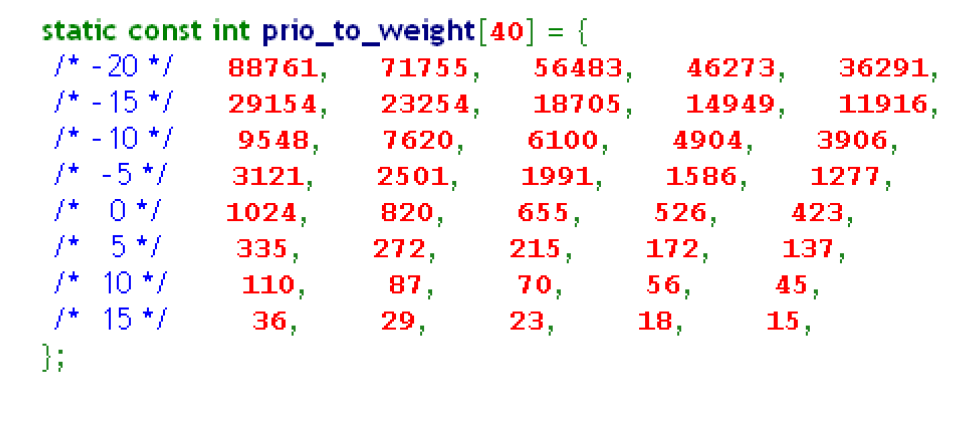
\includegraphics[width=10cm]{./figure/cfs_weight.png}
  \floatfoot{nice=0时,虚拟时间等于物理时间  }
  }
\end{figure}

所有虚拟时间挂在红黑树上,每次linux调度虚拟时间最小的进程运行。

\chapter{调整优先级}
\section{用 renice 改变进程优先级}
\section{用 nice 改变进程优先级}
\section{用 chrt 改变进程优先级}
\clearpage
%%% Local Variables:
%%% TeX-master: "main"
%%% End:
